\documentclass[a4paper]{article}


\usepackage{alphabeta} 
\usepackage{enumitem} 
\usepackage{mathtools}
\usepackage{amsmath, amssymb} 
\usepackage{amsthm}
\usepackage{cancel} 
\usepackage[margin=0.70in]{geometry} 
\geometry{left=3cm,right=3cm,top=2.4cm,bottom=2.4cm}	%the page geometry as defined, A4=210x297mm
\usepackage{graphicx}
\usepackage{wrapfig}
\usepackage{caption}
\usepackage{textcomp}
\usepackage{tabto}
\usepackage{layout}
\usepackage{bm}
\usepackage{minipage-marginpar}
\usepackage[dvipsnames]{xcolor}
\usepackage{hyperref}
\usepackage{dutchcal}
\usepackage{derivative}
\usepackage{esint}
%\usepackage{biblatex}
\usepackage{subcaption}
\usepackage{booktabs}\usepackage{derivative}
\usepackage[flushleft]{threeparttable}
\usepackage[capbesideposition=outside,capbesidesep=quad]{floatrow}
\usepackage{derivative}
\usepackage[thinc]{esdiff}
\usepackage{lipsum}
\usepackage{arydshln}
\usepackage[export]{adjustbox}
\usepackage{subcaption}
%%RENEW

\newtheorem{problem}{Άσκηση}
\newtheorem*{solution*}{Λύση}
\newtheorem{definition}{Ορισμός}[subsection]
\newtheorem{properties}{Ιδιότητες}[subsection]
\newtheorem{theorem}{Θεώρημα}[subsection]
\newtheorem{protash}{Πρόταση}[subsection]
\newtheorem{porisma}{Πόρισμα}[subsection]
\newtheorem{lemma}{Λήμμα}[subsection]
\newtheorem*{prooof}{Απόδειξη}
\newtheorem*{notes}{Παρατηρήσεις}
\newtheorem*{note}{Παρατήρηση}
\newtheorem*{app}{Εφαρμογή} 
\newtheorem*{example}{Παράδειγμα}
\newtheorem*{examples}{Παραδείγματα}


\newcommand\numberthis{\addtocounter{equation}{1}\tag{\theequation}}
%\renewcommand{\labelenumi}{\roman{enumi}}
\newcommand{\approxtext}[1]{\ensuremath{\stackrel{\text{#1}}{\approx}}}
\renewcommand{\figurename}{Εικόνα.}
\renewcommand{\tablename}{Πίνακας.}
%\renewcommand\refname{New References Header}
\renewcommand*\contentsname{Περιεχόμενα}
%\DeclareDerivative{\odv}{\mathrm{d}}


\begin{document}
\begin{titlepage}			%makes a title page. Remember to change the author, CID, username and group number to what is appropriate for you!
	\centering
	{\scshape\LARGE Εθνικό Μετσόβιο Πολυτεχνείο\par}
	{\scshape \LARGE Σ.Ε.Μ.Φ.Ε.\par}
	\vspace{1cm}
	{\huge\bfseries Οπτικές Ίνες \par}
	\vspace{1cm}
	{\Large\itshape Θωμόπουλος Σπύρος\par}		%remember to change these!
	
	%		{\large Group \@group\unskip\strut\par}
	{\large spyros.thomop@gmail.com/ ge19042@mail.ntua.gr\par \hfill \\}% 		%remember to change these!
	\vspace{1cm}
	{\large Ημερμονηνία Παράδοσης 04/04/2022\par}
\end{titlepage}

\subsection*{Σκοπός}
	Ο σκοπός της εν λόγω εργαστηριακής άσκησης είναι η μελέτη βασικών στοιχείων και φαινομένων που σχετίζονται με τις οπτικές ίνες όπως φαινόμενα διασποράς και εξασθένησης σήματος.
\subsection*{Θεωρητικά Στοιχεία}
	Μέσω των οπτικών ινών μπορούμε να μεταδίδουμε οπτικά σήματα με μεγάλη πυκνότητα πληροφορίας σε μεγάλες αποστάσεις. Ενδεικτικα, κάποια από τα θετικά τους είναι η μικρή διάμετρος, το μικρό βάρος, η υψηλη ευκαμπτότητά τους, το μεγάλο εύρος ζώνης. Αντίθετα, κάποια από τα αρνητικά των οπτικών ινών είναι ότι έχουν υψηλό κόστος εγκατάστασης και συντήρησης και είναι σχετικά εύθραυστες.
	\subsubsection*{Κατηγορίες Οπτικών Ινών}
		\subsubsection*{(I)Δείκτης Διάθλασης } 
			\textbf{Κλιμακωτές}\\
				Αποτελείται από έναν πυρήνα με δείκτη διάθλασης $n_1$ και ένα περίβλημα με $n_2$. Η συνθήκη για την διάδοση του φωτός εντός της οπτικής ίνας είναι να την εισάγουμε σε αυτή με γωνία μεγαύτερη ή ίση από την κρίσιμη γωνία ολικής εσωτερικής ανάκλασης. Επίσης, για να παρατηρείται ολική ανάκλαση κατά την διάδοση του σήματατος στον πυρήνα, θα πρέπει $n_1>n_2$. Ορίζουμε το \textit{αριθμητικό άνοιγμα (ΝΑ)} την ίνας  ως 
			\begin{align*}
				NA = n_1sin\theta_{in}	\numberthis
			\end{align*}	
και την \textit{κρίσιμη γωνία}			
			\begin{align*}
				sin\theta_c = n_2/n_1  		\numberthis
			\end{align*}
	Ο συνδυασμός περιβλήματος-πυρήνα μπορεί να είναι γυαλί-γυαλί, πλαστικό-γυαλί, πλαστικό-πλαστικό
				\\
			\textbf{Βαθμιαίες}\\
				Ο δείκτης διάθλασης του πυρήνα δεν είναι σταθερός, αλλά μειώνεται καθώς πηγαίνουμε προς το περίβλημα όπου και σταθεροποιείται ως εξής 
					\begin{align*}
						n(r) = n_1(1-(r/a)^2\Delta), &\text{ \gamma\iota\alpha }\hspace{0.1cm}r<a \\ 
						n(r) = n_1(1-\Delta)       , &\text{ \gamma\iota\alpha }\hspace{0.1cm}	r\geq a \numberthis
					\end{align*} 
			
			Οι αξονικές ακτίνες που διαδίδονται στο κέντρο έχουν μικρότερη ταχύτητα από τις περιφερειακές, αφού εκεί ο δείκτης διάθλασης είναι μεγαλύτερος με αποτέλεσμα να αντισταθμίζεται η μικρότερη απόσταση που διανύουν.
		\subsubsection*{(II) Πλήθος Διαδιδόμενων Ρυθμών}
			
			\textbf{Πολυρυθμικές}\\
				Έχουμε την διάδοση πολλών ρυθμών, δηλαδή ακτίνων διαφορετικών διευθύνσεων οι οποίες εισέρχονται στην ίνα με διαφορετικές γωνίες. Ισχύει ότι 
				\begin{align*}
					N = V^2/2 \\ 
					V = \pi d(NA)/\lambda 
				\end{align*}
					
			όπου d η διάμετρος του πυρήνα και $\lambda$ το μήκος κύματος της δέσμης. Παρατηρείται ακόμη, το φαινόμενο της \textit{διασποράς ρυθμών} που πρόκειται για την άφιξη των διαφορετικών ρυθμών στην έξοδο σε διαφορετικές χρονικές στιγμές.\\
					
		\textbf{Μονορυθμικές}
					
					Έχουμε διάδοση ενός ρυθμού για $V=2.405$ και κατ' επέκταση $d\leq2.405\lambda/\pi(NA)$. Εδώ προφανώς δεν παρατηρείται Διασπορά των Ρυθμών και γι' αυτό έχουμε και μεγαλύτερο Εύρος Ζώνης.
					
		\subsubsection*{Φαινόμενα Διασποράς}
			Κατά την έξοδο από την οπιτκή ίνα, ένας παλμός βγαίνει παραμορφωμένος. Υπάρχουν διάφορα είδη παραμόρφωσης και όλα οφείλονται σε φαινόμενα διασποράς, δηλαδή διαφορετικής ταχύτητας διάδοσης για διαφορετική συχνότητα. Όταν ένας μονοχρωματικός ρυθμός διαχωρίζεται σε ρυθμούς με διαφορετικούς χρόνους διάδοσης $\Delta \tau$ λέμε ότι έχουμε \underline{\textit{Διασπορά των Ρυθμών}}, με: 
			\begin{align*}
				\Delta \tau = \frac{(NA)^2}{2n_2c} , \hspace{1cm} v_{max} = \frac{1}{\Delta \tau}
			\end{align*}
			
			με $v_{max}$ το Εύος Ζώνης. \\ 
		Όταν παλμοί του ίδιου ρυθμού έχουν διαφορετικό μήκος κύματος τότε διαδίδονται σε διαφορετικές γωνίες και έχουμε \underline{\textit{Διασπορά του Κυματοδηγού}}. 
		\begin{align*}
			\Delta\tau = L\frac{n_1}{c}sin\theta\odv{\theta}{\lambda}\Delta\lambda
		\end{align*}
		
		όπου L το μήκος της ίνας, $\theta$ γωνία κώνου υποδοχής. \\ 
				Παλμοί διαφορετικού μήκους κύματος έχουν διαφορετικές ταχύτητες καθώς ισχύει ότι $n_2 = n_2(\lambda)$ και τότε έχουμε \underline{\textit{Διασπορά του Μέσου}}. 
		\begin{align*}
			\Delta\tau = L \frac{\lambda^2}{c} \odv[2]{n}{\lambda} \frac{\Delta\lambda}{\lambda}
		\end{align*}
		
		\subsubsection*{Εξασθένηση Σήματος}
			Κατά την διάδοση του σήματος σε μία οπτική ίνα παρατηρείται η μείωση της ισχύος του που προκαλεί την εξασθένηση L: 
			\begin{align*}
				L(dB) = 10log(\frac{P_{in}}{P_{out}})
			\end{align*}					
		
		Η εξασθένηση οφείλεται στην \textit{απορρόφηση} του σήματος από διάφορες προσμίξεις στο υλικό του πυρήνα και στην  \textit{σκέδαση} όταν το υλικό έχει ανομοιογένειες (γεωμετρικές ατέλειες, κάμψεις κατά την κατασκευή και το τύλιγμα της ίνας)
\subsection*{Πειραματική Διάταξη}
Γενικά, τα μέρη που θα χρειαστούμε σε όλα τα πειράμτα είναι 
	\begin{itemize}
		\item[.] Laser He-Ne 
		\item[.] Συζεύκτης laser-ίνας
		\item[.] Στήριγμα ίνας 
		\item[.] Οθόνη με χαρτί μιλλιμετρέ
		\item[.] Συζεύκτης ινών
	\end{itemize}
\subsection*{Πειραματική Διαδικασία - Επεξεργασία Μετρήσεων}

	\subsubsection*{Σύζευξη ίνας - laser}
		Θα μελετηθεί η σύζευξη μίας οπτικής ίνας με ένα laser He-Ne. Η σύζευξη επιτυγχάνεται με την παρουσία ενός συγκλίνωνα φακού ο οποίος λόγω φαινομένων περίθλασης δεν συγκεντρώνει την δέσμη σε ένα σημείο αλλά σε ομόκεντρους δίσκους  με Γκαουσιανή κατανομή. Για να είναι αποδοτική, θα πρέπει προφανώς η διάμετρος της ίνας να είναι μεγαλύτερη από αυτή της δέσμηςΗ ένταση της δέσμης μειώνεται με την απόσταση r που διανύει στην ίνα ως 
		\begin{align*}
			I = I_0 e^{-2 (\frac{r}{w})^2}
		\end{align*}
		w είναι η διάμετρος της δέσμης.
		
		Πιό ειδικά, ο συζεύκτης αποτελείται από το μέρος του φακού εστίασης και το μέρος της σύνδεσής του με την έξοδο του laser. Τα δύο μέρη συνδέονται μεταξύ τους και επιπλέον μπορούν να έχουν και διαφορετική κλίση η οποία αν ρυθμιστεί κατάλληλα μπορεί να εστιάσει την δέσμη στο κέντρο του πυρήνα και κατ' επέκταση όλη την ισχύ στο κέντρο του ίχνους της δέσμης σε μία οθόνη.
		
		Πειραματικά, αφού θέσουμε σε λειτουργία το laser, μετράμε με την φωτοδίοδο την τάση από το υπόβραθρο, το laser και της δέσμης του laser αφού το συνδέσουμε με την πολυρυθμική ίνα. Η μετατροπή της τάσης σε ισχύ γίνεται από την σχέση $P = -1.898 + 18.48 V(S.I.)$. Τα αποτελέσματα φαίνονται στον Πίνακα (\ref{mat1}) 
		\begin{table}[h!] 
			\centering 
			\begin{tabular}{|c|r|r|} \hline
				Μέτρηση & $V (V)$ & P(mW) \\ 
				\hline\hline
				Υπόβαθρο           & 0.345 & 4.48  \\ \hline
				Laser+ Υπόβαθρο    & 0.824 & 13.33 \\ \hline
				Ίνα  + Υπόβαθρο    & 0.650 & 10.11 \\\hline\hline
				Laser              & 0.479 & 6.95 \\\hline
				Ίνα                & 0.305 & 3.74  \\\hline
			\end{tabular}
			\caption{ }
			\label{mat1}
		\end{table}
		
		Τέλος, μπορούμε να υπολογίσουμε την εξασθένιση της οπτικής ίνας από την σχέση 
			\begin{align*}
				  &IL = 10log_{10} (\frac{P_{out}}{P_{in} }) = 10log_{10}(\frac{P_{Ίνα}	}{P_{laser}}) \Rightarrow \\ 
&\textcolor{white}{IL}= 10log_{10} (\frac{10.114}{13.330}) \Rightarrow\\
				   &\boxed{IL=-0.270}
			\end{align*}
	\subsubsection*{Προσδιορισμός Αριθμητικού Ανοίγματος}
		Μετρώντας την διάμετρο του ίχνους στην έξοδο της ίνας θα πορσδιορίσουμε το αριθμητικό άνοιγμά της. Συγκεκριμένα, τοποθετούμε την οθόνη με το μιλλιμετρέ χαρτί σε μία απόσταση από την έξοδο της ίνας και την απομακρύνουμε ανά 1cm. Σε κάθε βήμα μετράμε την διάμετρο. Τα αποτελέσματα φαίνονται στον Πίνακα (\ref{mat2}).
		\begin{table}[h!]
			\centering
			\begin{tabular}{|r|r|}%r|r|r|r|}
				\hline
				$x(\pm0.1cm)$ & $D(\pm0.1cm)$ \\%& $tan\theta$ & $\theta(^o)$ & $NA=sin\theta$ & $NA_{δέσμης}$ \\
				\hline\hline
				0.0 & 1.5 \\\hline %& $\infty$ & 90.0 & 1.00 & \\\hline
				1.0 & 2.1 \\\hline %& 1.05   & 46.4 & 0.72 & \\\hline
				2.0 & 2.7 \\\hline %& 0.68   & 34.0 & 0.56 & \\\hline
				3.0 & 3.2 \\\hline %& 0.53   & 28.1 & 0.47 & \\\hline
				4.0 & 3.6 \\\hline %& 0.43   & 23.0 & 0.39 & \\\hline 			
			\end{tabular}
			\caption{ }
			\label{mat2}
		\end{table}
		
		Όπου η γωνία $\theta$ είναι η γωνία του κώνου υποδοχής, δηλαδή η γνωία που σχηματίζει η ευθεία που ενώνει το κέντρο του ίχνους με την ίνα και η ευθεία που ενώνει ένα σημείο της περιμέτρου του ίχνους με την ίνα (Εικόνα (\ref{Im1})). Έτσι, θα δίνεται από την σχέση 
		\begin{align}\label{4}	
			tan\theta=D/2x
		\end{align}
		\begin{figure}[h!]
			\centering
			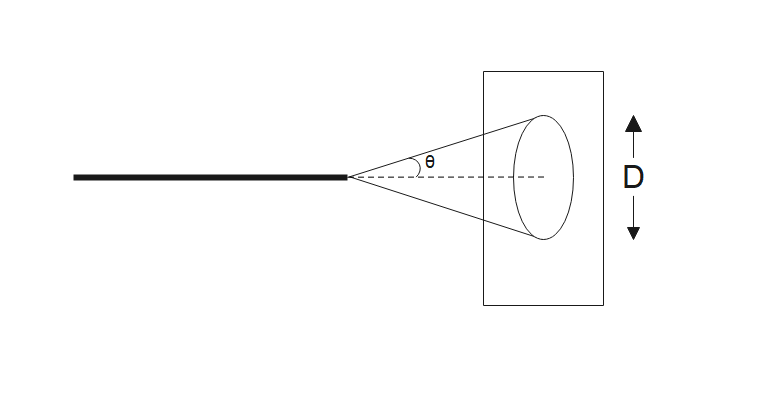
\includegraphics[scale=0.35]{konos_ypodoxhs.png}
			\caption{Γωνία Κώνου Υποδοχής}
			\label{Im1}
		\end{figure}
		
		Επιπλέον, το αριθμητικό άνοιγμα της δέσμης δίνεται από την σχέση 
	\begin{align}		
		NA_{δεσμης} = n_{αερα}sin\theta=\sqrt{n_{co}^2-n_{cl}^2} 
	\end{align}
	
	Άρα δεδομένου ότι η σχέση (\ref{4}) γράφεται $D = 2tan\theta\cdot x$, μπορούμε να εφαρμόσουμε μέθοδο ελαχίστων τετραγώνων για ευθεία της μορφής $Υ = ΑX+B$ \footnote{Το Β χρειάζεται γιατί το x που έχουμε ορίσει ως 0 δεν αντιστοιχεί σε μηδενική απόασταση από την έξοδο της ίνας. Αν είχαμε πάρει ως $x=0cm$ όταν η οθόνη βρισκόταν στην έξοδο της ίνας θα έπρεπε να χρησιμοποιήσουμε μία μέθοδο ελαχίστων τετραγώνων της μορφής $Y=AX$}, με $X = x$, $Y=D$ και  $A=2tan\theta$ και με αυτόν τον τρόπο να προσδιορίσουμε την γωνία $\theta$.
	 
	Από την εν λόγω μέθοδο προκύπτει   $A = (0.53\pm0.03)$, $B=(1.56\pm0.04)$ και η ευθεία με τα πειραματικά δεδομένα φαίνονται στην Εικόνα (\ref{Im2}) 
	
	\begin{figure}[h!]
		\centering
		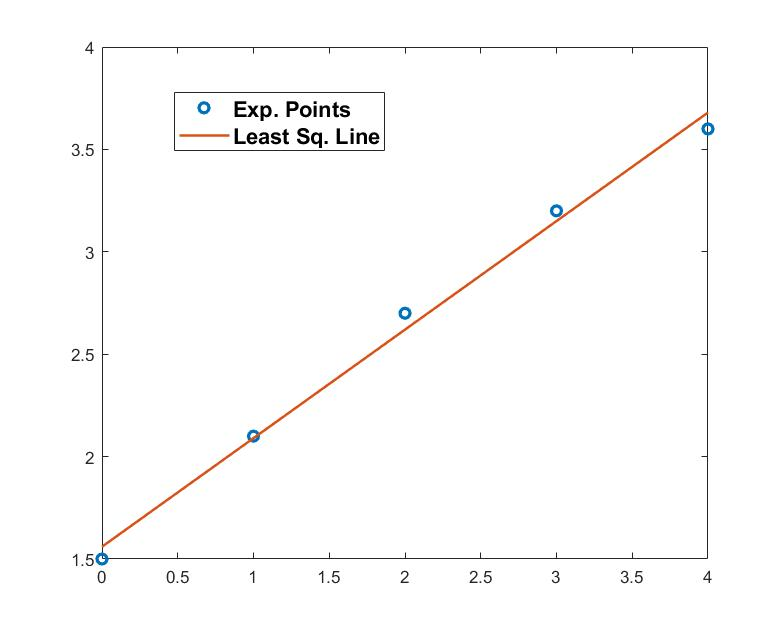
\includegraphics[scale=0.5]{NA.jpg}
		\caption{ }
		\label{Im2}
	\end{figure}
	
%	\footnotetext{Οι συντελεστές και τα σφάλματά τους πρκύπτουν από τις σχέσεις $A = \frac{\sum_{i=1}^{n}x_iy_i}{\sum_{i=1}^{n}x_i^2}$, $(\delta A)^2=\sigma_A^2=\frac{\sigma_y^2}{\sum_{i=1}^{n}x_i^2}$, $\sigma_y\simeq\sum_{i=1}^{n}\frac{(y_i-bx_i)^2}{n-1}$}
	
	Άρα για την γωνία θ έχουμε\footnotemark
		\begin{align*}
			\theta = ( 0.259\pm 0.024) [rad] = (14.8 \pm 1.4) ^o
		\end{align*}
	\footnotetext{Το σφάλμα προκύπτει από διάδοση $\delta\theta=|\pdv{\theta}{A}\delta A|=\frac{\delta A}{\sqrt{1+A^2/4}} =\frac{2\delta A}{\sqrt{4+A^2}}$}
	Τέλος το Αριθμητικό Άνοιγμα της ίνας είναι: \footnotemark
		\begin{align*}
			\boxed{NA = 0.26 \pm 0.02 }
		\end{align*}
		\footnotetext{Ομοίως το σφάλμα προκύπτει από διάδοση $\delta NA = |\pdv{sin\theta}{\theta}\delta\theta|=cos\theta\delta\theta$}
		
		
	\subsubsection*{Μετατροπή Δέσμης Εξόδου σε Παράλληλη}
		Εδώ θα χρησιμοποιήσουμε έναν οπτικό ευθυγραμμιστή(collimator), δηλαδή έναν συγκλίνωνα φακό ($f=1mm$), προκειμένου να παραλληλοποιήσουμε την δέσμη εξόδου της ίνας. Για να επιτυγχθεί αυτό θα πρέπει να τοποθετήσουμε την έξοδο της ίνας από τον φακό ίση με την εστιακή του f. 
		
		Αφού τοποθετήσουμε τον συζεύκτη στην έξοδο της ίνας, τον στρίβουμε μέχρι να γίνει ελάχιστο το μέγεθος του ίχνους της στην οθόνη. Όταν το επιτύχουμε αυτό θα έχουμε τοποθετήσει την έξοδο της ίνας στο εστιακό επίπεδο του φακού.
		
		Στρίβουμε τον φάκο κατά 180$^o$ (μία πλήρης περιστροφή μετακινεί τον φακό κατά 0.454mm).Η απόσταση του αντικειμένου (πυρήνας ίνας) είναι $o = f+(0.454/4 ) =1.114mm$  και η απόσταση του ειδώλου 
		\begin{align*}
			\frac{1}{f} = \frac{1}{o}+\frac{1}{i} \Rightarrow  \boxed{i = 9.772mm}
		\end{align*}
		Τότε η διάμετρος του ίχνους της δέσμης βρέθηκε $h_1=D=(5\pm1)mm$
		
	Γνωρίζουμε ότι η μεγέθυνση ενός αντικειμένου σε σύστημα ενός φακού δίνεται από την σχέση 
		\begin{align*}
			M = \frac{h_1}{h_0}=\frac{i}{o}\Rightarrow \\ 
			 h_0 = \frac{h_1\cdot o}{i} \Rightarrow \boxed{h_0=(0.6\pm 0.1) mm}\footnotemark 
		\end{align*}
		\footnotetext{Το σφάλμα προκύπτει από διάδοση $\delta h_0 = \sqrt{(\pdv{h_0}{h_1} \delta h_1)^2} = \frac{o}{i}\delta h_1 = 0.1139 \simeq 0.1mm$}
		
		Αρχικά πρέπει να σημειωθεί ότι έχουμε μεγάλο σχετικό σφάλμα της τάξης του $\sim 17\%$. Ακόμη, οι τιμές της διαμέτρου του πυρήνα για πολυρυθμική οπτική ίνα είναι $0.0500-0.0625mm$ και παρόλο που η τιμή μας δεν συμπίπτει με αυτές, δεν περιέχεται στα πλαίσια του σφάλματός της αφού πρόκειται και για διαφορετική τάξη μεγέθους. 
		
	\subsubsection*{Εξασθένηση κατά την Σύζευξη Δύο Ινών }
		
		Σε αυτό το μέρος θα μελετηθεί η σύζευξη δύο οπτικών ινών. Η σύζευξη επηρεάζεται από διάφορους παράγοντες όπως η \textit{πλευρική απόκλιση} (άξονες των ινών παράλληλα μετατοπισμένοι), \textit{γωνιακή απόκλιση} (άξονες των ινών σχηματίζουν γωνία), \textit{χωρισμός των άκρων}	(το φως που εξέρχεται από την πρώτη εισέρχεται στον κών υποδοχής της δεύτερης), \textit{κατεργασία άκρων} (επιφανειακές ατέλειες και ακαθαρσίες στα άκρα της ίνας), \textit{εσωτερικές απώλειες} (διαφορές στα οπτικά χαρακτηριστικά των ινών) και \textit{απώλειες Fresnel} (οφείλονται σε ανακλάσεις στις διαχωριστικές επιφάνειες).
		
		Αφού συνδέσουμε τις δύο ίνες, μετράμε με την φωτοδίοδο την τάση του υποβάθρου και έπειτα τις τάσεις που δίνει η έξοδος της ίνας όταν είναι τυλιγμένη μόνο η πρώτη και όταν είναι τυλιγμένες και οι δύο. Έπειτα μετατρέπεω τις τάσεις σε ισχύ σύμφωνα με την σχέση $P=-1.898+18.48V [S.I.]$. Ακόμη, υπολογίζω την εξασθένιση για τις δύο περιπτώσεις από την σχέση $IL=10log_{10}(P_{out}/P_{in})$, όπου είχαμε βρει την ισχύ του laser $P_{in}=P_{laser}=6.954mW$.Τα αποτελέσματα φαίνονται στον Πίνακα (\ref{mat3}).
		
		\begin{table}[h!]
			\centering 
			\begin{tabular}{|r|r|r|r|r|}
				\hline 
				Μέτρηση  			   & $V(V)$& P(mW) & IL(dB) \\ \hline\hline 
				Υπόβαθρο1			   & 0.442 & 6.27 & -  \\ \hline
				1η τυλιγμ. + Υπόβαθρο1 & 0.630 & 9.74 & -  \\ \hline
				Υπόβαθρο2              & 0.448 & 6.38 & -  \\ \hline
				2η τυλιγμ. + Υπόβαθρο2 & 0.596 & 9.12 & -  \\ \hline	
				\hline \hline 
				1η τυλιγμ.             & 0.188 & 1.58 & -6.45\\ \hline 
				2η τυλιγμ.             & 0.148 & 0.84 & -9.20\\ \hline
			\end{tabular}
			\caption{ }
			\label{mat3}
		\end{table}
		
	\subsubsection*{Συντελεστής Εξασθένησης της Ίνας}
		Η εξασθένιση των οπτικών ινών μετράται σε $dB/km$, την οποία και προκαλούμε με έναν τεχνητό εξασθενητή ο οποίος τοποθετείται ενδιάμεσα στις 2 ίνες. Οι μετρήσεις μας φαίνονται στον Πίνακα (\ref{mat4}).
		%Η ισχύς υπολογίζεται και πάλι από την σχέση $P_{in}=P_{laser}=6.954mW$.
		\begin{table}[h!]
			\centering
			\begin{tabular}{|r|r|r|r|}
				\hline
				$\#$ Στροφών $90^o$ & $V(mV)$     & $V-V_{back}(mV)$    & IL(dB) \\ 
				                  & (μετρήθηκε) & (από ίνα)  &        \\
				 \hline\hline 
				0 & $V_{in}=708$   & 296 &  -3.79 \\\hline
				1 & 683  		   & 271 &  -4.17 \\\hline
				2 & 645  		   & 233 &  -4.83 \\\hline
				3 & 611  		   & 199 &  -5.51 \\\hline
				4 & 574 		   & 162 &  -6.41 \\\hline
				5 & 514 		   & 102 &  -8.41 \\\hline
				6 & 479 	   	   & 67  &  -10.24\\\hline
				7 & $V_{back}=412$ & 0   &  --  \\\hline
			\end{tabular}
			\caption{ }
			\label{mat4}
		\end{table}
	
	Η γραφική παράσταση των παραπάνω μεγεθών προκύπτει έπειτα από προσαρμογή με πολυώνυμο 3ου βαθμού και φαίνεται στην Εικόνα 3: 
	
	\begin{figure}[h!]
		\centering
		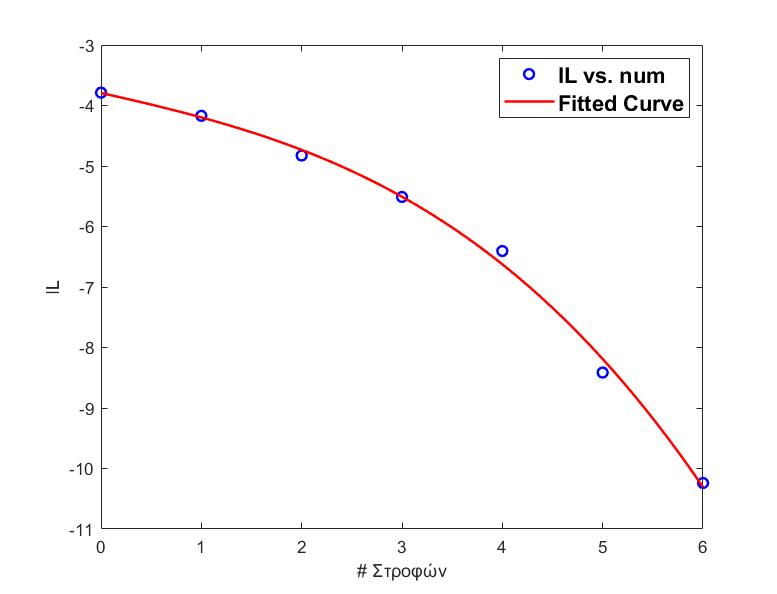
\includegraphics[scale=0.5]{last.jpg}
		\caption{ }
	\end{figure}
\subsection*{Συμπεράσματα}
\end{document}